\documentclass[10pt]{article}

% ── Packages ──────────────────────────────────────────────────────────────────
\usepackage[margin=1in]{geometry}
\usepackage{graphicx}
\usepackage{booktabs}
\usepackage{hyperref}
\usepackage{microtype}
\usepackage{parskip}
\usepackage{titlesec}
\usepackage{xcolor}
\usepackage{enumitem}
\usepackage{caption}
\usepackage{listings}
\usepackage{amsmath}

% ── Title formatting ───────────────────────────────────────────────────────────
\titlespacing*{\section}{0pt}{8pt}{4pt}
\titlespacing*{\subsection}{0pt}{6pt}{2pt}
\setlist[itemize]{noitemsep, topsep=2pt, leftmargin=*}

\hypersetup{colorlinks=true, linkcolor=blue, urlcolor=blue, citecolor=blue}

% ── Document ───────────────────────────────────────────────────────────────────
\begin{document}
\begin{titlepage}
    \begin{flushleft}
            \includegraphics[width=3cm]{logo_upna.jpg} % Ajusta el tamaño según necesites
        \end{flushleft}
    
    \begin{center}
        \vspace*{1cm}
            
        \Huge
        \textbf{Assignment 3: Document RAG System}
            
        \vspace{0.5cm}

        %\textbf{MULTI-LABEL TEXT CLASSIFICATION WITH BILSTM AND DISTILBERT}
        

         %\vspace{1cm}
        \LARGE
        NATURAL LANGUAGE PROCESSING 25/26
            
        \vspace{0.5cm}
        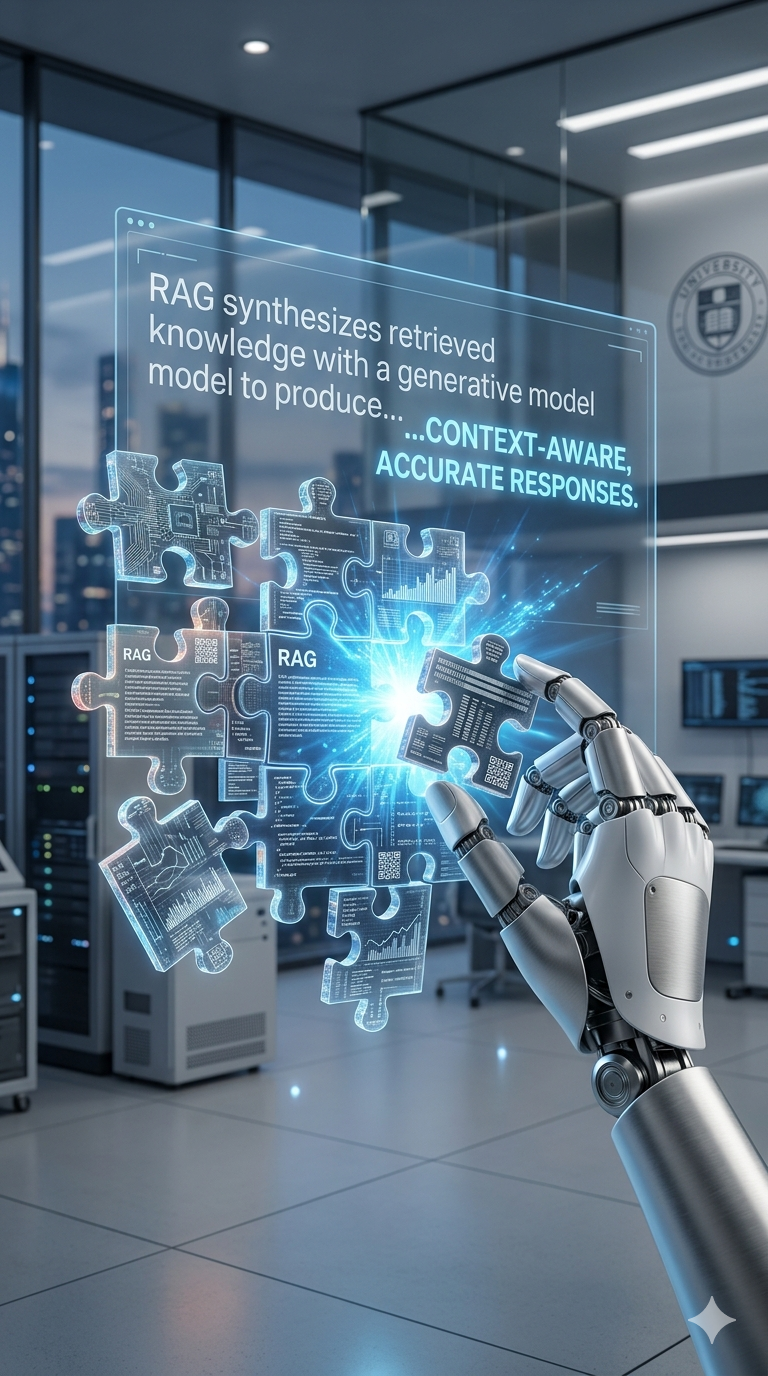
\includegraphics[width=12cm, height=12cm]{Imagen Portada.png}
        
            
        \vfill

        \vspace{0.5cm}
        \textbf{Roberto Aldanondo \& Andrés Malón}
        \vspace{0.5cm}
        
        {\large March 2026}
            
    \end{center}
\end{titlepage}

\vspace{6pt}

% ══════════════════════════════════════════════════════════════════════════════
\section{System Design}
% ══════════════════════════════════════════════════════════════════════════════

\subsection{Architecture Overview}

The system is a fully containerised Retrieval-Augmented Generation (RAG)
pipeline orchestrated with Docker Compose across five services:
MinIO (object storage), ChromaDB (vector database), a llama.cpp LLM server,
a Flask REST API, and a Streamlit frontend.
Figure~\ref{fig:arch} illustrates the data flow.

\begin{figure}[h]
  \centering
  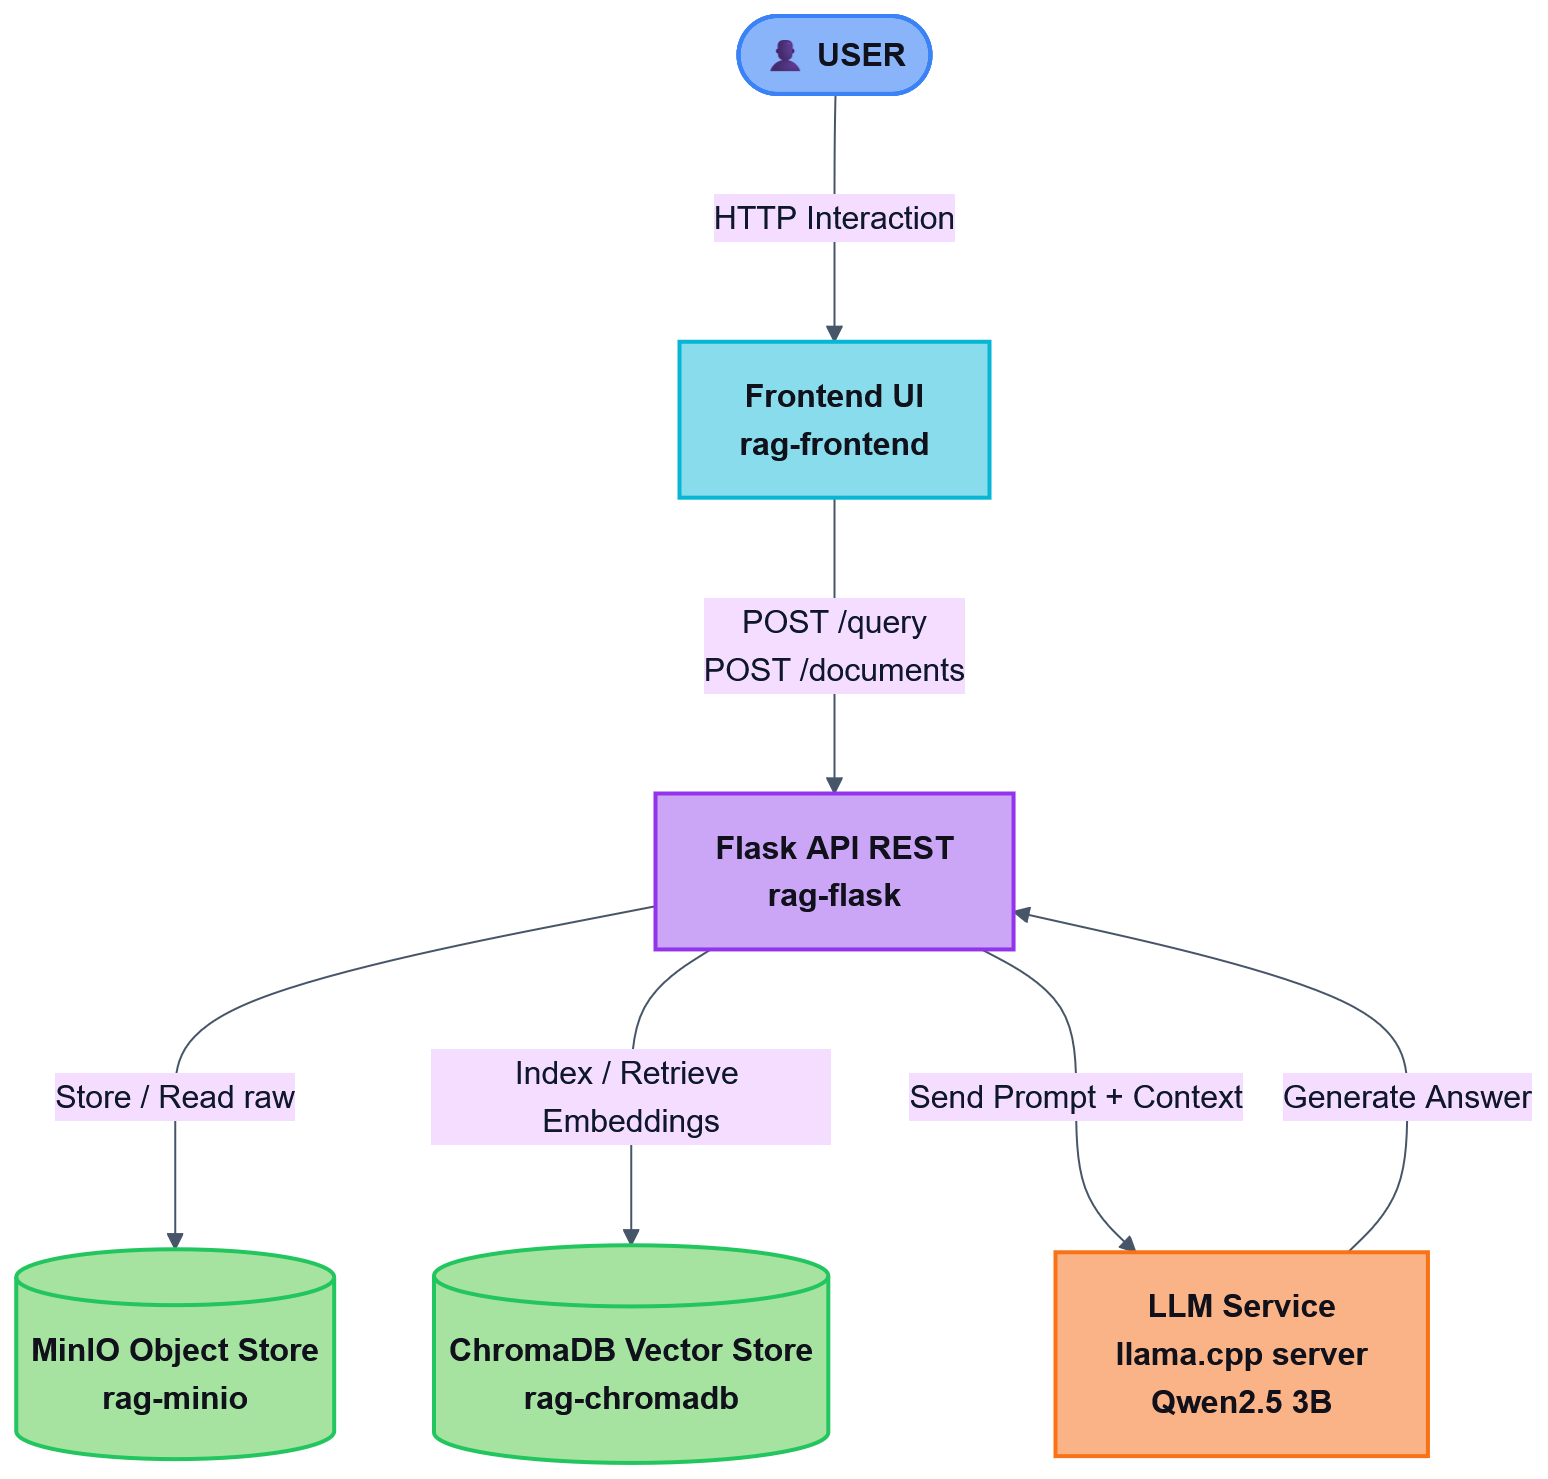
\includegraphics[width=\linewidth]{Diagrama Flujo Blanco.png}
  \caption{System architecture: five Docker services communicating
           over host networking. Arrows indicate the request/data flow
           for a user query.}
  \label{fig:arch}
\end{figure}

\noindent The ingestion pipeline (POST \texttt{/documents}) parses raw PDF or
DOCX files with \texttt{pdfplumber}/\texttt{python-docx}, chunks the
extracted text, embeds it, and upserts into ChromaDB in batches of 100.
Document metadata is stored in an embedded SQLite database.
Raw files are persisted in MinIO keyed as (\texttt{doc\_id/filename}) to
support future re-indexing.
Scanned image-only PDFs are detected by checking whether the extracted text
is shorter than 50 characters; in that case the API returns HTTP~422 with a
descriptive error rather than silently indexing an empty document.

\subsection{Infrastructure \& Container Orchestration}

All five services are declared in a single \texttt{docker-compose.yml} and
share \texttt{network\_mode: host}, which means every container binds directly
to the host's network stack and addresses the others via \texttt{localhost}.
This eliminates Docker's virtual bridge DNS overhead and, more importantly,
avoids the class of IP-resolution bugs that arise when containers reference
each other by service name while the embedding model is still loading.
The trade-off is reduced port isolation, which is acceptable for a local
research deployment.

Table~\ref{tab:services} summarises the five services and their ports.

\begin{table}[h]
\centering


\small
\begin{tabular}{@{}lll@{}}
\toprule
\textbf{Service} & \textbf{Image / Build} & \textbf{Port} \\
\midrule
MinIO      & \texttt{minio/minio:latest}           & 9000 / 9001 \\
ChromaDB   & \texttt{chromadb/chroma:latest}       & 8000 \\
LLM        & \texttt{ghcr.io/ggml-org/llama.cpp:server} & 8080 \\
Flask API  & Custom Dockerfile                     & 5000 \\
Streamlit  & Custom Dockerfile                     & 8501 \\
\bottomrule
\end{tabular}
\caption{Docker Compose service map.}
\label{tab:services}
\end{table}

\textbf{Health-check dependency chain.}
The \texttt{flask\_app} service declares
\texttt{condition: service\_healthy} on both MinIO and the LLM server,
and \texttt{condition: service\_started} on ChromaDB.
The LLM health-check polls \texttt{health} every 15s with a 30s
start-up grace period and up to 10 retries, covering the full model-load time
for a 2\,GB GGUF file on CPU.
MinIO is probed via \texttt{/minio/health/live} every 10\,s.
This chain guarantees that the Flask API never starts before its upstream
dependencies are ready, eliminating race-condition crashes that were the
primary stability issue during early development.

All configuration is injected via environment variables; no values are
hard-coded. The \texttt{Config} class reads every parameter---embedding model
name, chunk size, overlap, top-k, MinIO credentials, service hostnames---from
the environment, with safe defaults for local development.
This means the entire system can be reconfigured for a different deployment
(e.g.\ GPU host, different bucket name) by editing only \texttt{docker-compose.yml}.

\subsection{Component Rationale and Trade-offs}

Qwen2.5-3B-Instruct was chosen over larger alternatives (e.g.\ 7B models) for
two reasons: it fits within 4\,GB of system RAM when quantised to 4-bit
(Q4\_K\_M via GGUF), enabling stable CPU-only inference; and its instruction
fine-tuning delivers coherent, citation-aware answers for document Q\&A tasks
at this scale.
The llama.cpp server exposes an OpenAI-compatible
\texttt{/v1/chat/completions} endpoint, making the LLM backend trivially
swappable without changing application code.
The main trade-off is generation latency ($\sim$10--30\,s per query on CPU)
and a hard 256-token response budget that occasionally truncates long answers.
The context window is set to 4096 tokens (\texttt{-c 4096}) with
\texttt{--parallel 1} to avoid memory fragmentation on a single-core
inference path.

\textbf{Prompt Engineering.}
The system prompt is designed with strict constraints to ensure grounding.
The system message instructs the model to answer using \emph{only} the
provided context and to cite every claim as \texttt{[Source N]}; if the
context is insufficient the model must explicitly state it cannot answer
rather than hallucinate.
Context is injected as numbered passages, each prefixed with its filename
and chunk index so the user can trace every claim back to a specific document
location.
The per-source word budget is computed dynamically as
$\lfloor 800 / k \rfloor$ words (where $k$ is the number of retrieved
sources), keeping the total context under~1\,100 tokens while leaving room
for the 256-token response.
Generation uses temperature~0.3 and top-p~0.9 to balance factual fidelity
with fluent output.
When no documents have been uploaded, the prompt informs the model of the
empty knowledge base and instructs it to ask the user to upload documents
rather than generating from parametric knowledge.

\textbf{Chunking — Fixed-Size with Sliding Window (default) and Recursive
Splitting (alternative).}
Two strategies are implemented and selectable per upload via a \texttt{strategy}
form field.

\textit{Fixed-size} (default): a sliding window of 512 words advances in steps
of $512 - 50 = 462$ words, so consecutive chunks share a 50-word overlap.
The 512-word window fits comfortably within \texttt{BAAI/bge-base-en-v1.5}'s
effective context (512 subword tokens), while the overlap prevents
answer-bearing sentences near chunk boundaries from being silently discarded.
This strategy was retained as the default because it produces uniform chunk
lengths that are straightforward to reason about during evaluation.


\textit{Recursive splitting}: attempts to split text using a four-level
hierarchy of separators---paragraph break (\verb|\n\n|),
line break (\verb|\n|), sentence boundary (\verb|. |),
and word boundary (\verb| |)---applying the next finer separator only
when the current segment still exceeds \textit{max\_chunk\_size}.
This preserves the author's paragraph and sentence structure,
producing semantically more coherent chunks at the cost of variable lengths.

The known weakness of fixed-size chunking---arbitrary cuts through
mid-paragraph prose---is partially mitigated by the overlap.
The known weakness of recursive splitting---widely varying chunk sizes---can
cause uneven embedding density across the index.


\textbf{Retrieval — Bi-Encoder \texttt{BAAI/bge-base-en-v1.5} + ChromaDB.}
\texttt{BAAI/bge-base-en-v1.5} consistently outperforms
\texttt{all-MiniLM-L6-v2} on MTEB retrieval benchmarks while remaining
lightweight (109\,M parameters).
ChromaDB stores embeddings in an HNSW index with cosine distance, giving
sub-millisecond approximate nearest-neighbour search at this corpus scale.
The retriever over-fetches $3\times$ the requested \texttt{top\_k} and then
deduplicates by the first 200 characters of each chunk's text, which prevents
repeated chunks from duplicate document uploads from dominating the context
window.
The embedding model is cached in a global variable after the first load to avoid
reloading the 438 \, MB weights on every request.
No cross-encoder re-ranker is applied---a deliberate trade-off that avoids a
second inference pass at the cost of weaker precision@1.

\subsection{Flask REST API}

The Flask application exposes the five mandatory endpoints shown in
Table~\ref{tab:api}.

\begin{table}[h]
\centering

\small
\begin{tabular}{@{}lll@{}}
\toprule
\textbf{Method} & \textbf{Endpoint} & \textbf{Action} \\
\midrule
POST   & /documents        & Upload PDF/DOCX; returns doc ID \\
GET    & /documents        & List all docs with metadata \\
DELETE & /documents/\{id\} & Remove doc, chunks, MinIO object \\
POST   & /query            & Q\&A; returns answer + sources \\
GET    & /health           & Per-service liveness check \\
\bottomrule
\end{tabular}
\caption{REST API endpoint summary.}
\label{tab:api}
\end{table}

The ingestion flow on \texttt{POST /documents} is strictly ordered:
(1) validate file type; (2) parse text and detect scanned PDFs;
(3) upload raw bytes to MinIO; (4) chunk and embed; (5) upsert to ChromaDB;
(6) record metadata in SQLite.
If step 4-5 fails, the MinIO object is cleaned up to avoid orphaned files.

The query endpoint accepts an optional \texttt{top\_k} parameter
(default: 5) and returns the generated answer alongside a ranked list of
source passages, each carrying document ID, filename, chunk index, cosine
similarity score, and the first 500 characters of the chunk text.

The health endpoint probes MinIO, ChromaDB, the LLM server, and
the SQLite metadata store independently, returning HTTP~200 if all services
are reachable or HTTP~503 (with a per-service error map) if any are not.
This makes it suitable as the Docker health-check target for the Flask
container itself.

% ══════════════════════════════════════════════════════════════════════════════
\section{Retrieval Evaluation}
% ══════════════════════════════════════════════════════════════════════════════

\subsection{Evaluation Dataset}

The evaluation dataset is stored in \texttt{eval/eval\_dataset.json} and
follows the schema shown below:

\begin{itemize}
  \item \textbf{documents}: list of symbolic document descriptors, each with
        \texttt{doc\_id} (e.g.\ \texttt{eval\_doc\_1}), \texttt{filename}
 and a short description.
  \item \textbf{questions}: list of annotated questions, each with
        \texttt{id}, \texttt{question} text, \texttt{expected\_doc\_id}
        (pointing to the symbolic ID above), \texttt{expected\_answer}, and
        \texttt{relevant\_passage} (the verbatim excerpt that contains the answer).
\end{itemize}

The corpus comprises \textbf{7 documents} in total: 3 curated evaluation
documents spanning thematically distinct domains---an Artificial Intelligence
overview (PDF), a Climate Change report (PDF), and a Python Programming guide
(DOCX)---plus \textbf{4 real distractor documents} (NLP course assignments and
a CCTV technical report) indexed alongside the eval set to increase retrieval
difficulty.
\textbf{15 questions} span factual, conceptual, and definitional query types
(five per domain), evaluated at $k \in \{1, 3, 5\}$.

\subsection{Evaluation Methodology}

The evaluation script (\texttt{eval/run\_eval.py}) operates in five stages.

\textbf{Stage 1 — Document ID mapping.}
The eval dataset uses symbolic IDs (\texttt{eval\_doc\_1}, etc.), while the
live system assigns UUIDs at upload time.
The script calls \texttt{GET /documents} to retrieve the current document list
and maps each eval filename to its real UUID before metric computation.
This decoupling means the eval dataset does not need to be updated when
documents are re-uploaded.

\textbf{Stage 2 — Query execution.}
Each of the 15 questions is sent to \texttt{POST /query} with
\texttt{top\_k=5}.
The returned source list (up to 5 entries, ordered by cosine similarity)
is recorded for metric computation.

\textbf{Stage 3 — Metric computation.}
Three metrics are computed for each $k \in \{1, 3, 5\}$:

\begin{itemize}
  \item \textbf{Hit Rate@k}: fraction of queries where the expected document
        appears in the top-$k$ retrieved sources.
        $\text{HR}@k = \frac{1}{|Q|}\sum_{q} \mathbf{1}[\text{doc}_q \in
        \text{top}_k(q)]$
  \item \textbf{MRR@k}: mean reciprocal rank of the first occurrence of the
        expected document within the top-$k$ list.
        $\text{MRR}@k = \frac{1}{|Q|}\sum_{q} \frac{1}{\text{rank}_q}$
  \item \textbf{Precision@k}: fraction of the top-$k$ results that belong to
        the expected document.
        $\text{P}@k = \frac{1}{|Q|}\sum_{q} \frac{|\text{relevant} \cap
        \text{top}_k(q)|}{k}$
\end{itemize}

\textbf{Stage 4 — Qualitative sampling.}
The first three successes and up to two failures (at $k{=}3$) are logged with
their retrieved document ID lists and a preview of the generated answer.

\textbf{Stage 5 — Persistence.}
Full results---metrics, per-question pass/fail flags, retrieved ID lists,
and generated answers---are saved to \texttt{results/eval\_results.json}.

\subsection{Quantitative Results}

\begin{table}[h]
\centering
\caption{Retrieval metrics on the 15-question evaluation set
         with 7 documents in the index (3 eval + 4 distractors).}
\label{tab:metrics}
\small
\begin{tabular}{@{}lccc@{}}
\toprule
\textbf{k} & \textbf{Hit Rate} & \textbf{MRR} & \textbf{Precision} \\
\midrule
@1 & 0.800 & 0.800 & 0.800 \\
@3 & 0.867 & 0.833 & 0.511 \\
@5 & 1.000 & 0.867 & 0.347 \\
\bottomrule
\end{tabular}
\end{table}

The system achieves perfect recall at $k{=}5$ despite having 4 thematically
related distractor documents in the index.
MRR@5 of 0.867 indicates the relevant document lands at rank~1 for the
majority of queries; the drop from HR@1 (0.800) to HR@3 (0.867) reveals
exactly 2 queries where the correct document was recovered only at rank~4.
Precision decreases naturally with $k$ as more distractor chunks enter the
retrieved set.

At $k{=}1$, 12 out of 15 questions retrieved the correct document as the
top result. The 3 remaining questions all reached the correct document by
$k{=}5$, confirming there are no complete retrieval failures in the corpus---
every relevant chunk is reachable, but for 2 queries the bi-encoder ranks
distractor chunks higher.

\subsection{Qualitative Analysis}

\textbf{Success case 1 — Definitional query.}
\textit{``What is the Turing Test?''} retrieved the AI overview as rank-1.
Qwen2.5-3B produced a grounded answer citing Alan Turing (1950) and the
human-evaluator test design, with no hallucinated claims.
The query's specificity (a proper noun unique to the AI document) made it
trivial for the bi-encoder.

\textbf{Success case 2 — Factual query.}
\textit{``What are the main causes of climate change?''} retrieved the
Climate Change document at rank~1.
The model correctly identified fossil fuel combustion and deforestation
as primary drivers, citing Source~1.
The domain-specific vocabulary (``greenhouse gas'', ``fossil fuels'') strongly
differentiated the climate document from the distractors.

\textbf{Failure case 1 — Distractor interference (NLP domain overlap).}
\textit{``What is transfer learning in AI?''} failed at $k{\leq}3$.
The top-3 results were dominated by the NLP course assignment distractor
documents, which contain dense machine-learning terminology
(transformers, fine-tuning, BERT) that is semantically closer to the query
embedding than the simpler AI overview chunk.
The correct document only appeared at rank~4.
This is the most instructive failure: real-world distractor collections
that share vocabulary with the query domain are the primary challenge for
bi-encoder retrieval without re-ranking.

\textbf{Failure case 2 — Broad query ambiguity.}
\textit{``What is natural language processing?''} also failed at $k{\leq}3$.
NLP is a central topic in the distractor assignments, causing three
distractor chunks to outscore the AI overview chunk.
The correct document recovered only at rank~4, and the LLM (lacking
the right chunk in its context window) produced a partially hallucinated
answer by extrapolating from adjacent ML content in the distractor passages.

% ══════════════════════════════════════════════════════════════════════════════
\section{Reflection}
% ══════════════════════════════════════════════════════════════════════════════

\subsection{What Worked Well}

\textbf{Docker Compose orchestration.}
Declaring all five services in a single \texttt{docker-compose.yml} with
host-mode networking dramatically simplified dependency management.
Health checks ensured the LLM server was fully loaded before the Flask API
accepted traffic, eliminating race-condition crashes that caused silent
failures during early development when the model file was still being read
from disk.
The \texttt{restart: on-failure} policy on the Flask container provided
a safety net for any transient startup errors.

\textbf{Embedding model quality.}
\texttt{BAAI/bge-base-en-v1.5} proved robust even against semantically
related distractor documents. Achieving HR@5 = 1.00 on a 7-document corpus
with 4 NLP-themed distractors---without any cross-encoder re-ranking---
confirms the bi-encoder's discriminative power at this scale.
The decision to over-fetch $3\times$ and deduplicate before returning results
further improved effective precision by eliminating redundant chunks from
repeated uploads.

\textbf{Model migration.}
The system was initially prototyped with TinyLlama-1.1B-Chat-Q4\_K\_M, which
produced incoherent answers and frequent hallucinations.
Switching to Qwen2.5-3B-Instruct-Q4\_K\_M required only updating the model
path in \texttt{docker-compose.yml} and renaming the model field in
\texttt{llm\_client.py}, with zero changes to the rest of the codebase---
validating the modular architecture.

\textbf{Modular API design.}
Separating ingestion, chunking, retrieval, and generation into distinct
Python modules (\texttt{ingestion.py}, \texttt{chunking.py},
\texttt{retrieval.py}, \texttt{llm\_client.py}) made each component
independently testable and replaceable.
The \texttt{Config} class centralises all runtime parameters as
environment-variable reads with safe defaults, making the system portable
across machines without code changes.

\textbf{Grounding contract enforcement.}
The explicit system-prompt instruction to refuse answering when context is
insufficient proved effective: in cases where the retriever returned wrong
chunks, the model's response was a clear ``I cannot fully answer this based
on the provided documents'' rather than a confidently wrong answer.
This aligns with the expected behavior of a reliable Q\&A system..

\subsection{What Did Not Work Well}

\textbf{LLM context truncation causing generation failures.}
Even when the retriever returned the correct document at rank~1, the LLM
sometimes responded that it could not fully answer the question.
Investigation revealed that the 800-word context budget split
across 5 sources limits each chunk to $\sim$160 words, which can cut off
the specific sentence that answers the question.
Queries like \textit{``What is a Python decorator?''} and
\textit{``How does exception handling work?''} suffered from this: the correct
chunk was retrieved but its answer-bearing sentence fell beyond the 160-word
cutoff.
This is a generation failure, not a retrieval failure, caused by the
interaction between a small \texttt{max\_tokens} budget and a large
\texttt{top\_k}.

\textbf{Distractor-driven retrieval failures.}
The two HR@3 failures (\textit{transfer learning}, \textit{NLP}) were caused
by real NLP assignment documents in the index.
These distractors contain denser and more recent ML vocabulary than the
synthetic eval documents, making them higher-scoring for broad AI queries.
A bi-encoder without re-ranking cannot distinguish ``this document is about
NLP in general'' from ``this document specifically answers this query''.

\textbf{Fixed-size chunking at semantic boundaries.}
Word-count boundaries are agnostic to paragraph structure.
Chunks spanning two distinct topics dilute the embedding centroid, as
observed in the transfer learning failure where a chunk containing both
a discussion of feature extraction and an unrelated definition of backpropagation
produced an embedding that matched neither query well.

\textbf{SQLite metadata store volatility.}
The metadata database is stored in the container's filesystem at
\texttt{/app/metadata.db}. Without a named Docker volume for this path,
a container restart deletes all document metadata while ChromaDB and MinIO
(which use host-path volumes) retain their data. This causes a state
inconsistency where documents exist in the vector index and object store
but are invisible to the API.

\subsection{Proposed Future Improvements}

Three targeted improvements would address the observed failures directly.

\textbf{(1) Reduced top-k with larger per-chunk budget.}
Reducing \texttt{top\_k} to~3 and raising \texttt{max\_tokens} to~512 would
resolve the LLM context truncation issue without any architectural change.
The trade-off is lower recall at the retrieval stage, which would need to be
monitored.

\textbf{(2) Semantic chunking.}
Replacing fixed-size chunking with semantic chunking--splitting on cosine
similarity drops between consecutive sentences--would produce topic-coherent
chunks, directly addressing the transfer learning and NLP retrieval failures
by preventing vocabulary from unrelated topics from diluting a chunk's
embedding centroid.

\textbf{(3) Cross-encoder re-ranker.}
Adding a lightweight cross-encoder
(e.g.\ \texttt{cross-encoder/ms-marco-MiniLM-L-6-v2}) as a second-stage
filter over the top-15 bi-encoder results would push HR@1 toward $>$ 0.93
for the distractor failure cases, because a crossencoder jointly encodes
query and passage and is therefore more sensitive to relevance nuance.

\textbf{(4) Persistent SQLite volume.}
Mounting \texttt{/app/metadata.db} to a named Docker volume would resolve the
metadata volatility issue and keep the API's document list consistent with the
vector index across container restarts.

\subsection{Bonus: Streamlit Frontend UI}

A multi-tab Streamlit interface was implemented.
It provides: (1) a drag-and-drop document upload panel with chunking strategy
selection; (2) a document library with per-document metadata (filename, upload
date, chunk count, strategy) and one-click deletion; and (3) a persistent chat
interface with expandable source citations showing filename, chunk index, and
cosine similarity score.
A sidebar health-check panel reports the live status of all four backend
services by polling \texttt{GET /health}, which proved invaluable during
debugging when services were partially degraded.
The frontend is containerised with its own Dockerfile and declared as the
fifth service in \texttt{docker-compose.yml}, reachable at port~8501.


\section*{Code Repository}
The full source code is available at:
\url{https://github.com/andresmln/Assigment_3}

\end{document}
